\documentclass[twoside]{article}

\usepackage[a4paper, total={674pt, 426pt}, landscape]{geometry}
\usepackage{multicol}

\newcommand{\todo}[1]{\textcolor{red}{\textbf{TODO:} #1}}
\newcommand{\dyade}[1]{\overleftrightarrow{#1}}
\newenvironment{definition}[1]{\begin{tcolorbox}[title=Def.: #1, colback=white!,colframe=green!50!black]}{\end{tcolorbox}}

\titlespacing*{\section}{0pt}{.6\baselineskip}{.1\baselineskip}
\titlespacing*{\subsection}{0pt}{.6\baselineskip}{.1\baselineskip}
\titlespacing*{\subsubsection}{0pt}{.6\baselineskip}{.1\baselineskip}


%% This is the space for custom commands for your Formelsammlung
\newcommand{\FormelsammlungTitel}{High-frequency, Components, Amplifiers and Oscillators}
\newcommand{\FormelsammlungAutor}{Bogdan Stamenic}
\setcounter{tocdepth}{2} % Show only sections and subsection in table of contents

\begin{document}
	\title{\FormelsammlungTitel}
	\author{\FormelsammlungAutor}
	\date{\today}
	\begin{multicols}{3}
        \maketitle
        \tableofcontents
        \section{Wave Parameters and Passive High-Frequency Components}
\begin{itemize}
    \itemsep0pt
    \item Scattering matrix $S$:
        \[\begin{bmatrix}b_1\\ b_2\end{bmatrix} =\
            \begin{bmatrix}S_{11} & S_{12}\\ S_{21} & S_{22}\end{bmatrix} \
            \begin{bmatrix}a_1\\ a_2\end{bmatrix}\]
            \item \textbf{Symmetry:} \(\left(S = S^\top\right) \land \left(S_{ii} = S_{jj}\;\;\forall\:i, j \in \left[1;\:\mathrm{dim}\{S\}\right]\,\right)\)
                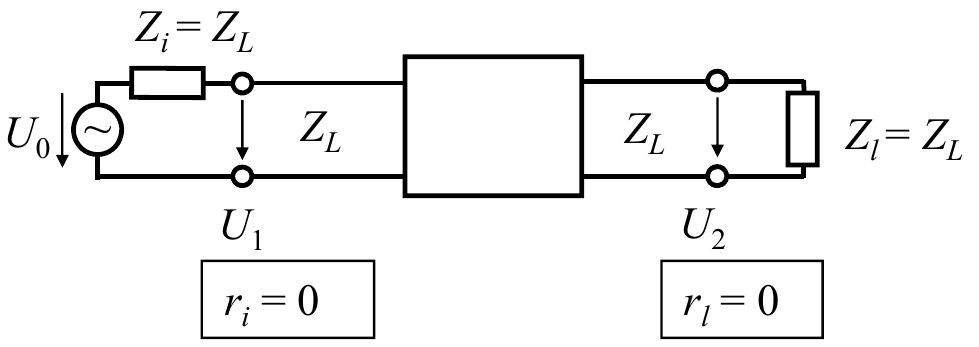
\includegraphics[width=.3\paperheight]{content/hfcomp/pictures/general_two-port.png}
    \item For a general 2-port, the following holds:
        \begin{flalign*}
            &S_{21} = 2 \dfrac{U_2}{U_0} \sqrt{\dfrac{Z_1}{Z_2}},\;\; S_{12} = 2 \dfrac{U_1}{U_0} \sqrt{\dfrac{Z_2}{Z_1}},\\
            &U_{f1} = \dfrac{U_0}{2},\;\; g_T = |S_{21}|^2,\;\; \dfrac{U_2}{U_1} = \dfrac{S_{21}}{(1 + S_{11})}
        \end{flalign*}
    \item For \(Z_{L1} \neq Z_{L2}\), all of the above equations hold, if $U_f$ and $U_b$ are replaced by \textit{normalized power wave amplitudes}:
        \begin{align*}
            &a_i = \dfrac{U_{fi}}{\sqrt{Z_{Li}}} &b_i = \dfrac{U_{bi}}{\sqrt{Z_{Li}}}
        \end{align*}
\end{itemize}

\subsection{Even/Odd Exitation of Symmetric Circuits}
\begin{itemize}
    \itemsep0pt
    \item Split a symmetric circuit into two less complex circuits
    \item \textit{Even(+)}-mode: in-phase excitation at both ports
    \item \textit{Odd(-)}-mode: excitation with opposite phases at both ports
    \item S-parameters of the original four-port are formally found to be:
        \begin{align*}
            S_{11} &= \dfrac{1}{2} (S_{11,e} + S_{11,o}),\\
            S_{21} &= \dfrac{1}{2} (S_{21,e} + S_{21,o}),\\
            S_{31} &= \dfrac{1}{2} (S_{21,e} - S_{21,o}),\\
            S_{41} &= \dfrac{1}{2} (S_{11,e} - S_{11,o}),\\
        \end{align*}
\end{itemize}

\subsection{Wilkinson Divider}
\begin{center}
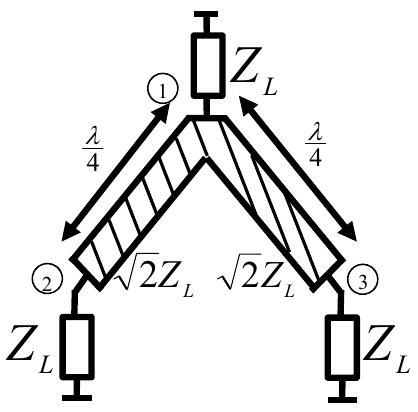
\includegraphics[width=3cm]{content/hfcomp/pictures/lossless_wilkinson_divider.png}
\end{center}
\begin{itemize}
    \itemsep0pt
    \item Input power is equally divided among the output ports, without reflections at the input port
    \item Scattering matrix with(-out) transverse resistor:
        \begin{align*}
            &\text{Without (lossless):} & S &= \
            \begin{bmatrix}\
                0 & \frac{-j}{\sqrt{2}} & \frac{-j}{\sqrt{2}}\\\
                \frac{-j}{\sqrt{2}} & \frac{1}{2} & \frac{-1}{2}\\\
                \frac{-j}{\sqrt{2}} & \frac{-1}{2} & \frac{1}{2}\
            \end{bmatrix}\\
            &\text{With (lossy):} & S &= \dfrac{-j}{\sqrt{2}}\
            \begin{bmatrix}\
                0 & 1 & 1\\\
                1 & 0 & 0\\\
                1 & 0 & 0\
            \end{bmatrix}\\
        \end{align*}
\end{itemize}

\subsection{Transmission Line Hybrid Coupler}
\begin{itemize}
    \itemsep0pt
    \item When \textit{fed at one port}, one output port is \textit{decoupled} and the other two output ports have \textit{equal amplitude}, but \textit{different phase differences} dependant on the design
    \item Most often: \ang{90}-hybrid, \ang{180}-hybrid Rat-Race
    \item Scattering matrix of \ang{90}-hybrid coupler with coupling factor $k$:
        \begin{align*}
            S &=
            \begin{bmatrix}\
                0 & k & -j\tau & 0\\\
                k & 0 & 0 & -j\tau\\\
                -j\tau & 0 & 0 & k\\\
                0 & -j\tau & k & 0\
            \end{bmatrix}\\
            \tau &= \sqrt{1 - k^2}
        \end{align*}
\end{itemize}

\subsection{Coupled Transmission Lines}
\begin{itemize}
    \itemsep0pt
    \item Unshielded transmission lines (in close proximity) are electromagnetically coupled $\implies$ directional couplers and bandpass filters can be realized
    \item Transmission line model with \textit{coupling capacitor} (elec. coupling) and \textit{coupling inductor} (magn. coupling)
%        \begin{align*}
%            &\frac{\mathrm{d}I_1}{\mathrm{d}z} = -j\omega(C^\prime_1 + C^\prime_{12})U_1 + j\omega C^\prime_{12}U_2\\
%            &\frac{\mathrm{d}I_2}{\mathrm{d}z} = -j\omega(C^\prime_2 + C^\prime_{12})U_2 + j\omega C^\prime_{12}U_1\\
%            &\frac{\mathrm{d}U_1}{\mathrm{d}z} = -j\omega L^\prime_1 I_1 - j\omega M^\prime I_2\\
%            &\frac{\mathrm{d}U_2}{\mathrm{d}z} = -j\omega L^\prime_2 I_2 - j\omega M^\prime I_1\\
%            &k = \frac{M^\prime}{L^\prime}\text{ (coupling coef.)}
%        \end{align*}
    \item For a transformer (inductive coupling):
        \begin{minipage}{.3\paperheight}
            \begin{circuitikz}[>=stealth, straight voltages, scale=.65, transform shape]
    \draw (0,0) node[transformer core, american](T){}
    %%Transformer primary side
    (T.A1) node[]{}
    +(-.5,0) node[ocirc]{} to[short, i=$I_1$] (T.A1)
    (T.A2) node[]{}
    +(-.5,0) node[ocirc]{} to[short] (T.A2)
    (T.A1)++(-.5,0) to[open, v=$U_1$] +(0,-2)
    %%Transformer secondary side
    (T.B1) node[]{}
    +(.5,0) node[ocirc]{} to[short, i^=$I_2$] (T.B1)
    (T.B2) node[]{}
    +(.5,0) node[ocirc]{} to[short] (T.B2)
    (T.B1)++(.5,0) to[open, v=$U_2$] +(0,-2);
    \draw [to-to] (T.inner dot A1) to[out=60, in=120] node[anchor=south]{$M$} (T.inner dot B1);
    \draw[-{Implies}, double, thick] (2,0) -- (2.5,0);
    \begin{scope}[xshift=7.5cm, yshift=0cm]
        \draw
        (0,0) node[transformer](G){}
        (G.A1) node[ocirc]{}
        to[short] +(-1,0)
        (G.A2) node[ocirc]{}
        to[short] +(-1,0)
        (G.B1) node[ocirc]{}
        (G.B2) node[ocirc]{};
        \path
        (G.inner dot A1) -- node[anchor=south]{$n:1$} (G.inner dot B1);
        \draw
        (G.A1)+(-1,0) to[L, *-*, american inductors, L=$k^2 L_1$]
        +(-1,-2.1);
        \draw
        (G.A1)++(-1,0) to[L, american inductors, L=$(1-k^2)L_1$] +(-2.5,0) node[ocirc]{}
        +(0,-2.1) to[short] +(-2.5,-2.1) node[ocirc]{};
%        ++(0,-2) to[short]
%        ++(-2,0) node[ocirc]{};
    \end{scope}
\end{circuitikz}

        \end{minipage}
        \begin{align*}
            &n = \dfrac{M}{L_2}, \quad k = \dfrac{M}{\sqrt{L_1 L_2}}\text{ (coupl. coeff.)},\\
            &\begin{bmatrix}\
                U_1\\
                I_1
            \end{bmatrix}\
            =\
            \begin{bmatrix}\
                n & 0\\
                0 & 1/n
            \end{bmatrix}\
            \begin{bmatrix}\
                U_2\\
                -I_2
            \end{bmatrix} \parbox{2cm}{(ideal trafo)}\\
            &L_1\text{: primary coil inductance}\\
            &L_2\text{: secondary coil inductance}
        \end{align*}
\end{itemize}

\subsection{Signal Flow Graphs}
\begin{itemize}
    \itemsep0pt
    \item Connection of wave amplitudes ($U_f$, $U_b$, $a$, $b$) by \textit{symbolic graph representation}
    \item \textbf{Vertex (knot):} wave amplitude
    \item \textbf{Branch:} transmission coefficient $S_{ij}$
    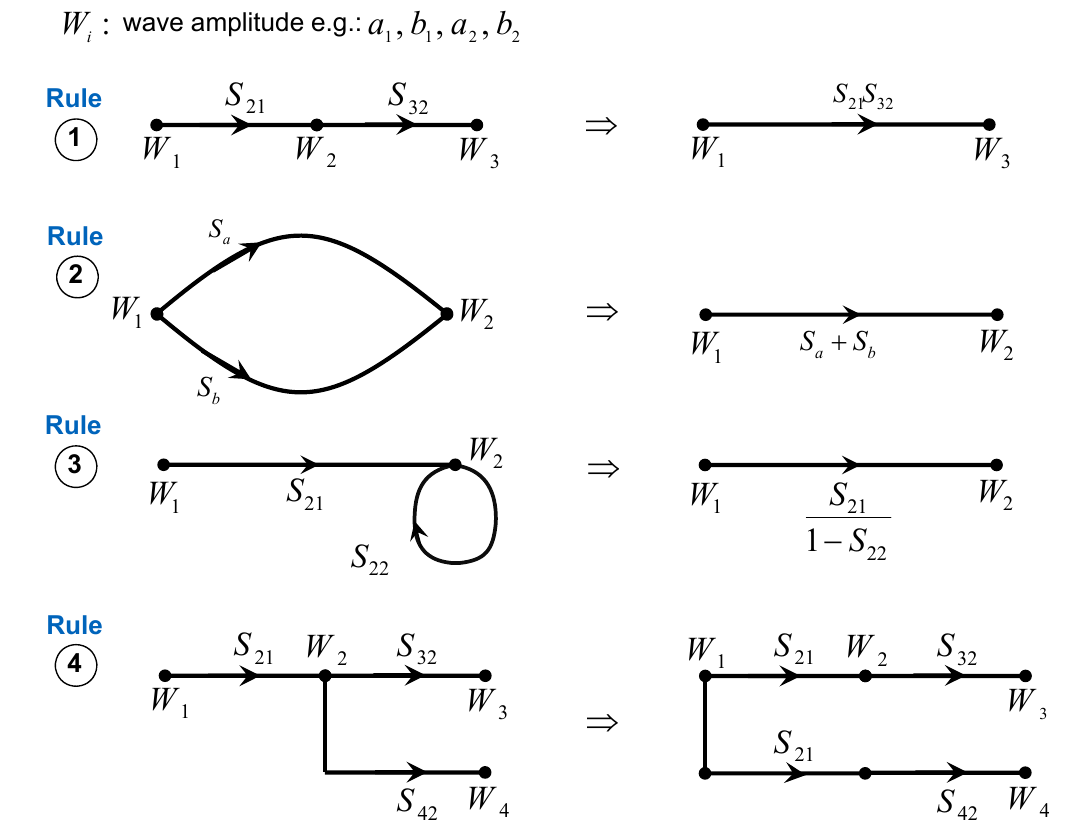
\includegraphics[width=.3\paperheight]{content/hfcomp/pictures/rules_signal_flow_graph.png}
    \item \textbf{Simplification rules for signal flow graphs:}
        \begin{enumerate}
            \item \(W_3 = S_{21}S_{32} W_1\)
            \item \(W_2 = W_1 S_a + W_1 S_b\)
            \item \(W_2 = W_1 \dfrac{S_{21}}{1 - S_{22}}\)
            \item Signal flow must not be changed!!!
        \end{enumerate}
    \item Analysis by Mason's Gain Rule:
        \begin{itemize}
            \itemsep0pt
%            \item \textbf{Independant variable:} Vertex of incident wave ($U_{fi}$, $a_i$)
%            \item \textbf{Dependant variable:} Vertex of an outgoing wave ($U_{bi}$, $b_i$)
            \item \textbf{Path:} Propagation path from an independant vertex ($a_i$) to a dependant vertex ($b_i$)following the positive direction of the branches, such that no vertex is passed more often than once.
            \item \textbf{Path Value:} Product of the branch coefficients of all branches along the path.
            \item \textbf{Loop of first order $L(1)$:} Product of the branch coefficients on a closed loop from one vertex back to the same vertex without passing any vertex twice.
            \item \textbf{Loop of second order $L(2)$:} Product of \textit{two loops of first order}, which do not touch (not even in a vertex).
            \item \textbf{Loop of third order $L(3)$:} Product of \textit{three loops of first order}, which do not touch (not even in a vertex).
            \item \textbf{Mason's Gain Rule:}
                \begin{align*}
                    &T = \dfrac{P_1 \xi_1 + P_2\xi_2 + P_3\xi_3 +...}{1 - \sum L(1) + \sum L(2) - \sum L(3) + ...},\\\\
                    &\xi_i = \left(1 - \sum L(1)^i + \sum L(2)^i - ...\right),\\
                    &L(1)^i:\parbox{4cm}{loops of order 1 that don't touch path $P_i$}
                \end{align*}
        \end{itemize}
\end{itemize}

\subsection{Non-Reciprocal Ferrite  Components}
\begin{itemize}
    \itemsep0pt
    \item In general: \(\mu_r = \mu_r^\prime - j\mu''_r\)
    \item YIG-Filter ($Y_3 Fe_2 O_{12}$) $\implies$ $H_0$ controls filter behaviour; selectively choose for left-/right-handed polarization
    \item \textit{Faraday Rotation} due to different permeabilites for left-/right-handed circ. pol. waves due to gyro-magnetic effects
    \item Uni-line circulator uses Faraday rotation to realize \textit{one-way} transmission line
    \item Y-Circulator (3-port) used to decouple transmitter-antenna-receiver for high powers
\end{itemize}

        \section{Active Circuit Elements}
\subsection{HF Diodes}
\subsubsection{Schottky Diodes}
\begin{itemize}
    \itemsep0pt
    \item n-type semiconductor; better carrier mobility of electrons
    \item Small barrier capacitance $\implies$ \textit{Fast switching}
    \begin{equation*}
        \text{Characteristic curve: }i = I_0 \left(\mathrm{exp}\left(\dfrac{u}{U_T} - 1\right)\right)
    \end{equation*}
\end{itemize}

\subsubsection{Capacitance/Varactor Diode}
\begin{itemize}
    \itemsep0pt
    \item Reverse biased p-n-diode; application of reverse voltage causes a barrier
    \item Increasing voltage $\to$ decreasing capacitance
    \item Can be used as an \textit{electronically variable capacitance}
    \item \textbf{Application:} tuning of resonators, filters, ...
\end{itemize}

\subsubsection{Tunnel Diode}
\begin{itemize}
    \itemsep0pt
    \item The u-i-characteristic exhibits regions with \textit{negative differential resistance}
    \item Can be used for the \textit{amplification of high-frequency} signals
    \item \(G_{n} \downarrow \left(|U|\uparrow \right)\)
\end{itemize}

\subsubsection{Impatt Diode}
\begin{itemize}
    \itemsep0pt
    \item Written out: \textbf{imp}act ionization \textbf{a}valanche \textbf{t}ransit \textbf{t}ime
    \item Negative differential resistance
    \item Usage in high-power applications
    \item Amplifier/Oscillator
    \item \textbf{Drawback:} high phase noise from avalanche effect
    \item Operation as a \textit{read diode}:
        \begin{align*}
            \Theta = \omega t = \omega \; w/v_s\\
            I_D = I_{\mathrm{max}} \dfrac{\Theta}{\pi} e^{-j\Theta/2} \dfrac{\sin\Theta/2}{\Theta/2}
        \end{align*}
    \item \(R_n \downarrow \left(|U_s|\uparrow\right)\)
    \item Operation up to \SI{94}{GHz}
\end{itemize}

\subsubsection{PIN Diode}
\begin{itemize}
    \itemsep0pt
    \item \textit{Positive-intrinsic-negative} diode
    \item Constant charge can be achieved by impressing a current \(|I_{DC}| = \left|\dfrac{dQ_x}{dt}\right|\)
    \item Properties:
        \begin{itemize}
            \itemsep0pt
            \item Fast switching times between high resistance and short circuit \(\approx \SI{1}{ns}\)
            \item linearly variable HF resistance
            \item Low insertion loss
            \item High break-through voltage due to large length of intrinsic zone possible
        \end{itemize}
    \item Use cases:
        \begin{itemize}
            \itemsep0pt
            \item Electronic switching element
            \item Variable $\pi$-attenuator with input-output matching to a real wave impedance
        \end{itemize}
\end{itemize}


\subsubsection{Gunn Element}
\begin{itemize}
    \itemsep0pt
    \item The Gunn Element is \textit{not} a diode
    \item Oscillator/Amplifier
    \item \textbf{Justification:} \textit{negative differential mobility} of the electrons (negative resistance/conductance)
\end{itemize}

\subsection{HF-Transistors}
\fbox{%
    \parbox{8cm}{%
        \textbf{Two-step analysis of HF-Transistor Amplifier Circuits:}
        \begin{enumerate}
            \itemsep0pt
            \item DC-analysis around quiescent point $\implies$ calculate resistances
            \item Small signal analysis using HF equivalent circuit
        \end{enumerate}
    }
}
\subsubsection{Bipolar Transistor}
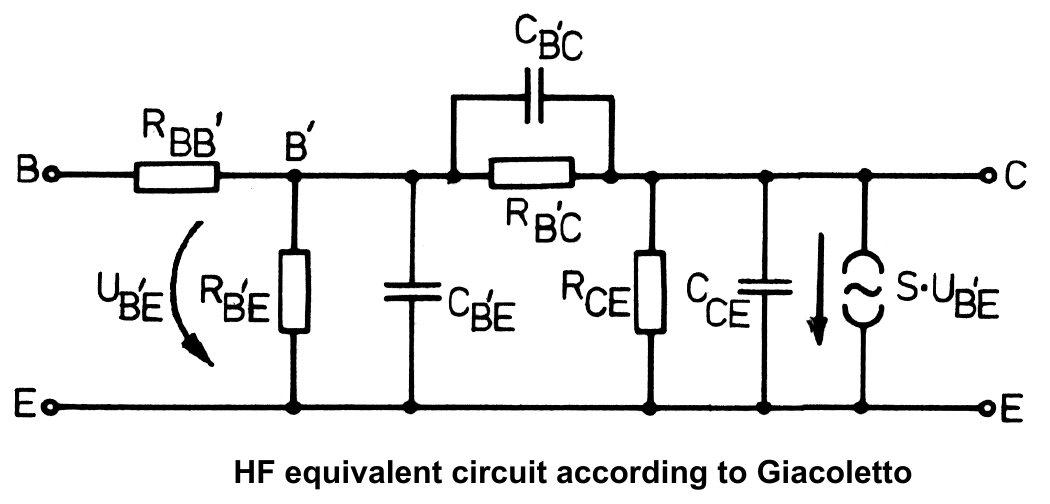
\includegraphics[width=.3\paperheight]{content/hfcomp/pictures/bipolar_transistor_giacoletto.png}
\begin{align*}
    &S \approx \dfrac{I_{E,DC}}{U_T}, \quad C_{B^\prime E} \approx \dfrac{S}{2\pi f_T},\\
    &\dfrac{1}{R_{B^\prime E}} = G_{B^\prime E} \approx \dfrac{S}{\beta_0},\\
    &\beta_0 = \left.\dfrac{I_C}{I_B}\right|_{f\to0} \approx \dfrac{I_{C,DC}}{I_{B,DC}} = B,\\
    &U_T = \frac{k_B T}{q_e}, \; U_T(T=\SI{25}{\degree C}) \approx \SI{25}{mV}\\
    &f_T\text{: transit frequency }(\beta = 1),\\
    &B\text{: DC current amplification},\\
    &k_B\text{: Boltzmann constant},\\
    &T\text{: Abs. temperature in Kelvin},\\
    &q_e\text{: Elementary charge}
\end{align*}
\begin{itemize}
    \itemsep0pt
    \item The HF operational parameters depend on the chosen operating point. The following is also achieved:
    \begin{itemize}
        \itemsep0pt
        \item \textit{Control} and \textit{stabilization} of the HF operational parameters
        \item Compensation of \textit{device tolerances}
        \item \textbf{Principle:} DC current feedback circuit
    \end{itemize}
\item E12-series resistors:
    \begin{equation*}
        R_n = 10^\frac{n}{12} 10^p \quad n=0,1,2,...
    \end{equation*}
\end{itemize}

\subsubsection{Field-effect Transistor}
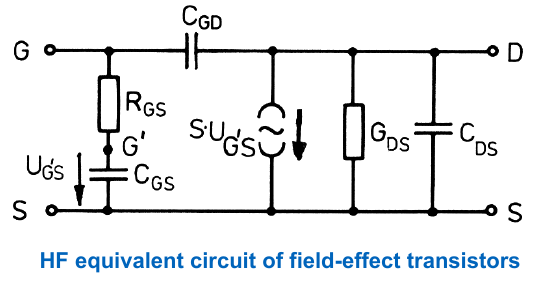
\includegraphics[width=.3\paperheight]{content/hfcomp/pictures/mosfet_hf_equivalent.png}\\
n-channel MOSFET, depletion type:
\begin{align*}
    &i_D \approx I_{DSS} \left(1 - \dfrac{u_{GS}}{U_P}\right)^2\\
    &S = \left.\dfrac{\partial i_D}{\partial u_{GS}}\right|_{U_{DS}=\mathrm{const}} = \dfrac{2}{|U_P|}\sqrt{I_{DSS} \; i_D}\\
    &U_P\text{: pinch-off voltage, here } U_P < 0
\end{align*}

\subsection{Microwave Tubes}
\subsubsection{Klystron}
\begin{itemize}
    \itemsep0pt
    \item Continuous electron beam is velocity modulated by an HF signal $\implies$ density-modulation
    \item Density modulated beam equivalent to an AC current $\implies$ excites \textit{amplified} oscillation in output resonator
\end{itemize}
\begin{align*}
    &i \approx I_0 \left(1 + p \cos(\omega t_0)\right)\\
    &p = \dfrac{\omega l |U_e|}{2v_0 U_0}\text{ (bunching parameter)}
\end{align*}

\subsubsection{Travelling Wave Tube (TWT)}
\begin{itemize}
    \itemsep0pt
    \item Density modulated electrons, as with Klystron
    \item Energy transfer \textit{only if}(!) average electron velocity $v_0$ is greater than the phase velocity $v_p$ of the RF wave $\implies$ delay lines for RF wave
\end{itemize}
\begin{align*}
    &v_p \approx c_0 \sin \psi, \quad v_p < v_0\\
    &\psi\text{: angle of helical delay line}
\end{align*}

\subsubsection{Magnetron (ger.: Kreuzfeldröhre)}
\begin{itemize}
    \itemsep0pt
    \item Similar to Klystron and TWT, but additionally \textit{shaped by DC magnetic field}
    \item Electron beam excites resonators embedded in the cathode
\end{itemize}

        \section{HF Amplification}
\begin{itemize}
    \itemsep0pt
    \item \textbf{Transmitter:} amplification of the oscillator power
    \item \textbf{Receiver:} amplification of the received power
    \item Small signals (pre-amplification): \textit{small distortions} (lower efficiency) are preffered
    \item Larger signal (power amplifier): \textit{efficiency} is more important
\end{itemize}

\subsection{Pre-Amplification}
\begin{itemize}
    \itemsep0pt
    \item Transducer power gain (Betriebsleistungsverstärkung):
        \begin{equation*}
            g_T = |A_B|^2 = \dfrac{P_2}{P_{i,\mathrm{max}}} = \dfrac{\frac{1}{2}|U_2|^2 R_i}{\frac{1}{2}|\frac{U_0}{2}|^2 R_2}
        \end{equation*}
    \item Transmittance (Betriebsübertragungsfaktor):
        \begin{align*}
            &A_B = \dfrac{U_2}{U_0 / 2}\sqrt{\dfrac{R_i}{R_2}} = |A_B| e^{-jb_B},\\
            &b_B\text{: transmission phase}
        \end{align*}
    \item Attenuation (Betriebsdämpfung):
        \begin{equation*}
            a_B = -20\,\lg |A_B| \quad [\si{dB}]
        \end{equation*}
    \item Group delay time:
        \begin{equation*}
            \tau_g = \dfrac{\mathrm{d}b_B}{\mathrm{d}\omega}
        \end{equation*}
\end{itemize}

\subsection{Power Ampflification}
\begin{equation*}
    \eta = \dfrac{P_t}{P_I} \quad \text{(efficiency)}
\end{equation*}
\begin{itemize}
    \itemsep0pt
    \item FETs and Tubes offer \textit{almost powerless control}
    \item Different operation modes  depending on the \textit{DC operating point} $\implies$ Class A, B, C,... operation
    \item \textit{Linearity/efficiency trade-off!}
    \item \textbf{Class A Operation}
        \begin{align*}
            &U_{G,DC} = U_{G0}/2, \quad U_1 = -U_{G,DC},\\
            &\theta_a = \ang{180},\\
            &\eta = \dfrac{P_t}{P_I} = 0.5\text{ (theor. max.)}
        \end{align*}
    \item \textbf{Class B Operation}
        \begin{align*}
            &U_{G,DC} = U_{G0}, \quad |U_1| = -U_{G,DC},\\
            &|I_a| = 0.5 \, I_{\mathrm{max}}, \quad I_{a,DC} = 0.318 \, I_{\mathrm{max}},\\
            &\theta_a = \arccos\left(1-U_{G0}/U_{G,DC}\right) = \ang{90},\\\\
            &\eta = \dfrac{P_t}{P_I} = \dfrac{1}{4\cdot0.318} = 0.786\text{ (max.) }\\
            &\implies \text{No loss for zero input signal!}
        \end{align*}
    \item \textbf{Class C Operation}
        \begin{align*}
            &U_{G,DC} = 2 U_{G0}, \quad |U_1| = -U_{G,DC},\\
            &|I_a| = 0.393 \, I_{\mathrm{max}}, \quad I_{a,DC} = 0.218 \, I_{\mathrm{max}},\\
            &\theta_a = \ang{60},\\\\
            &\eta = \dfrac{P_t}{P_I} = 0.9\text{ (max.) }
        \end{align*}
\end{itemize}

\subsection{Two-Terminal (1-Port) Amplifier}
\begin{itemize}
    \itemsep0pt
    \item Diodes with negative coductivity, e.g. tunnel diode\\
        \begin{tikzpicture}
            \begin{scope}[xshift=-1cm]
                \draw (0,0)node[ocirc]{} to[stroke diode, v^=$U$, i=$i$] (0,2)node[ocirc]{};
            \end{scope}
            \begin{scope}[xshift=1cm, scale=.8, transform shape]
                \draw (0,2)node[ocirc]{} to[R=$R_s$] (2,2) to[L=$L_s$, american] (4,2) to[C=$C_D$] (4,0) to[short] (0,0)node[ocirc]{};
                \draw (4,2) to[short, *-] (5.5,2) to[xgeneric, l=$-R_n$] (5.5,0) to[short, -*] (4,0);
                \draw[-{Stealth}] (0,1)node[fill=white!]{$Z$} -- (1,1);
            \end{scope}
        \end{tikzpicture}
\end{itemize}

        \section{Electronic Noise}
\begin{itemize}
    \itemsep0pt
    \item Noise: \textit{threshold for the perception of a signal}
    \item \textbf{Signal-to-noise ration:} \(\dfrac{S}{N} = \dfrac{P_S}{P_N}\)
    \item Limits of perceptibility:
        \begin{itemize}
            \item Analogue speech signal: $\text{NL} \approx 0\si{dB}$
            \item Analogue TV signal $\text{NL} \approx 34\si{dB}$
            \item With apriori and correlation techniques \(\implies \text{NL} < 0\si{dB}\)
        \end{itemize}
    \item \textbf{Noise sources}:
        \begin{itemize}
            \item Thermal noise $\propto T$ (resistors)
            \item Shot noise $\propto q_e I_{DC}$ (active/biased elements)
            \item Antenna noise: man-made, atmospheric (lightning) and cosmic (CMB)
        \end{itemize}
\end{itemize}

\subsection{Properties of Noise Signals}
\begin{itemize}
    \item Temporal behaviour is fundamentally \textit{unpredictable} $\implies$ integral values are predictable:
        \begin{align*}
            &\text{Linear, time average:}\\
            &\bar{u}^{\Delta t} = \dfrac{1}{\Delta t}\int\limits^{t_0+\Delta t}_{t_0} u(t) \mathrm{d}t\\
            &\text{Mean square:}\\
            &\overline{u^2}^{\Delta t} = \dfrac{1}{\Delta t}\int\limits^{t_0+\Delta t}_{t_0} u^2(t) \mathrm{d}t\\
            &\text{Root Mean Square (RMS):}\\
            &\tilde{u}=\sqrt{\overline{u^2}}
        \end{align*}
    \item Wide sense stationarity assumed; $\bar{u}^{\Delta t}$ and $\overline{u^2}^{\Delta t}$ independant from $t_0$
    \item Spectral density of voltage: \(W_u^s = \left.\dfrac{\bar{u}^2}{\Delta f}\right|_{\Delta f \to 0}\)
    \item \textbf{Central Limit Theorem} (Gaussian PDF):
        \(p^*(u) = \dfrac{1}{\sqrt{2\pi\:\overline{u^2}}}\exp\left(- \dfrac{1}{2}\dfrac{u^2}{\overline{u^2}}\right)\)
    \item \textbf{(Normalized) Error Function:}
        \begin{align*}
            p(0<u<u_1) &= \int\limits_0^{u_1} p^*(u)\mathrm{d}u =\\
            &= \Phi^*\left(\dfrac{u_1}{\tilde{u}}\right) \approx \dfrac{1}{2} - \dfrac{\exp(-\frac{1}{2}\frac{u_1^2}{\tilde{u}^2})}{\sqrt{2\pi}(u_1/\tilde{u})}
        \end{align*}
        \begin{tabular}{|c|c|c|c|c|}\hline
            $\dfrac{u_1}{\sqrt{\overline{u^2}}}$ & 1 & 2 & 3 & 4\\\hline
            $\Phi^*$ & 0.413 & 0.4772 & 0.4987 & 0.49997\\\hline
        \end{tabular}
\end{itemize}

\subsection{Working with Noise Signals}
\subsubsection{Correlation Functions}
\begin{itemize}
    \itemsep0pt
    \item Auto- ($i=j$)/Cross- ($i\neq j$)\textbf{Correlation Function}:
    \begin{align*}
        \rho_{ij}(\tau) &= \overline{u_i(t) u_j(t+\tau)}\\
        &= \lim_{\Delta t\to\infty} \dfrac{1}{\Delta t} \int\limits^{t_0+\Delta t}_{t_0} u_i(t) u_j(t+\tau) \mathrm{d}t
    \end{align*}
    \item $\rho_{ii}(\tau) = \rho_{ii}(-\tau) \implies \text{Even function!}$
    \item $\rho(0) = \sqrt{\overline{u^2}} = \tilde{u}$ (RMS)
    \item However, cross-correlation function $\rho_{ij}(\tau)$ \textit{not generally even!}
\end{itemize}

\subsubsection{Noise Signals in Frequency Domain}
\begin{align*}
    &\overline{u^2} = \int\limits_0^\infty W_u^s(f) \mathrm{d}f = |\tilde{u}|^2\\
    &W_u^s\text{: single-sided (power) spectral density}
\end{align*}
\begin{itemize}
    \itemsep0pt
    \item Double-sided spectral densities (\textit{even function}) as Fourier transform of correlation functions:
        \begin{align*}
            W_u(f) &= \int\limits^\infty_{-\infty}\rho(\tau)\,e^{-j2\pi f\tau}\mathrm{d}\tau\\
            &= \int\limits^\infty_{-\infty}\rho(\tau) \cos(-j2\pi f\tau)\mathrm{d}\tau\\
        \end{align*}
    \item \textbf{Wiener-Khinchin-Relations:}
    \begin{align*}
        &W_{u12} = \int\limits^\infty_{-\infty}\rho_{12}(\tau)\,e^{-j2\pi f\tau}\mathrm{d}\tau,\\
        &W_{u12}(f) = W_{u21}^*(f),\\
        &W_{u21}(f) = W_{u21}^*(-f)
    \end{align*}
    \item Normalized cross spectral density $\gamma$:
        \begin{equation*}
            \gamma = \dfrac{W_{u12}(f)}{\sqrt{W_u1(f)} \sqrt{W_u2(f)}}
        \end{equation*}
\end{itemize}

\subsubsection{Noise Signals in Linear Networks}
\begin{tabular}{cc}
    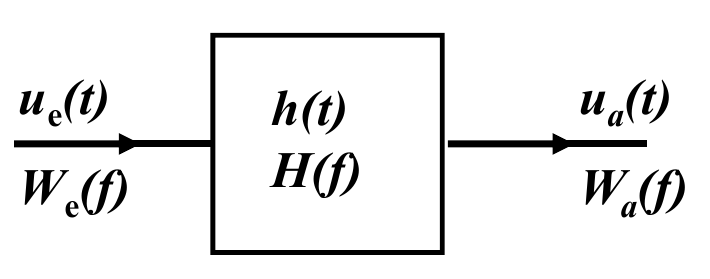
\includegraphics[width=3.5cm]{content/hfcomp/pictures/2-port_linear_network.png}\
    &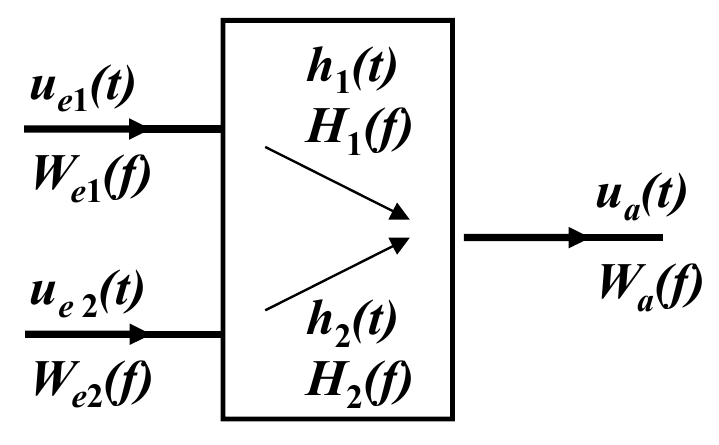
\includegraphics[width=3.5cm]{content/hfcomp/pictures/3-port_linear_network.png}\\
\end{tabular}
\begin{itemize}
    \itemsep0pt
    \item Two-port network with tranfer function $h(t)$:
        \begin{align*}
            &\rho_a(\tau) = \int\limits_{-\infty}^\infty\int\limits_{-\infty}^\infty\
            h(t')h(t'')\rho_e(\tau+t'-t'')\mathrm{d}t'\mathrm{d}t'',\\
            &W_a(f) = |H(f)|^2 W_e(f),\\
            &\rho_e\text{: Input autocorrelation function}\\
            &\rho_a\text{: Output autocorrelation function}
        \end{align*}
%    \item Three-port network (2 in-, 1 output) with tranfer functions $h_{1/2}(t)$:
%        \begin{align*}
%            W_a(f) = &|H_1(f)|^2 W_{e1}(f) + |H_2(f)|^2 W_{e2}(f)\\
%            &+ 2\:\mathrm{Re}\{H_1^*(f) H_2^*(f) W_{e1e2}(f)\}
%        \end{align*}
\end{itemize}
\fbox{%
    \parbox{7.5cm}{%
        \textbf{Symbolic Calculation of Noise Sources:}
        \begin{enumerate}
            \item Treat noise sources like normal current/voltage sources and apply Kirchhoff's laws to combine sources, e.g.
                \begin{equation*}
                    U_a = H_1(f)U_{e1} + H_2(f)U_{e2}.
                \end{equation*}
            \item Take the magnitude squared of the expression and apply the correspondence $|\tilde{U}_{e1}|^2 = W_{e1}$ for voltage or $|\tilde{I}_{e1}|^2 = W_{e1}$ for current sources, e.g.
                \begin{align*}
                    |U_a|^2 = &|H_1|^2|U_{e1}|^2 + |H_2|^2|U_{e2}|^2\\
                    &+ 2\:\mathrm{Re}\{H_1^* H_2^*\:U_{e1}^* U_{e2}\},\\
                    \updownarrow\\
                    W_a(f) = &|H_1|^2 W_{e1} + |H_2|^2 W_{e2}\\
                    &+ 2\:\mathrm{Re}\{H_1^* H_2^*\:W_{e1e2}\}.
                \end{align*}
        \end{enumerate}}
    }

\subsection{Noise of Two-Terminal Elements}
\subsubsection{Thermal Noise}
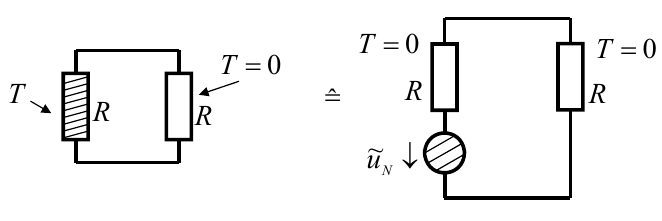
\includegraphics[width=.33\paperheight]{content/hfcomp/pictures/thermal_noise_resistor.png}
\begin{align*}
    &\overline{u^2(t)} = 4k_B T R\,\Delta f = |\tilde{u}|^2\\
    &W_{tu}^s(f) = 4\,k_B T\,R \quad \text{(single-sided)}\\\\
    &P_{N\;\mathrm{max}} = \dfrac{\overline{u^2(t)}}{4}\dfrac{1}{R} = k_B T\Delta f\\
    &\dfrac{P_{N\;\mathrm{max}}}{\mathrm{W}} = 4\cdot10^{-21}\;\dfrac{\Delta f}{\mathrm{Hz}}\dfrac{T}{T_0}
\end{align*}

\subsubsection{Noise of Receiving Antennas}
\begin{itemize}
    \itemsep0pt
    \item Equivalent antenna noise temperature $T_a=T$ (like a \textit{black body})
    \item Sources:
        \begin{itemize}
            \itemsep0pt
            \item cosmic noise
            \item atmospheric noise (tropical thunderstorms)
            \item ionospheric (fluctuation) noise
            \item heat radiation of the earth received by low directivity antennas
        \end{itemize}
\end{itemize}

\subsubsection{Shot Noise}
\begin{itemize}
    \itemsep0pt
    \item Due to the \textit{quantisation of electric charge}
    \item \textbf{Shottky equation} (derived from considering high vacuum diode):
        \begin{align*}
            W_{is}^s(f) = 2q_e\,q_e n |S(f)|^2 \approx 2 q_e\,I_{\mathrm{DC}}
        \end{align*}
\end{itemize}

\subsection{Noise of Diodes}
\begin{center}
    \begin{circuitikz}[scale=.8, transform shape]
    \begin{scope}[scale=1.2, xshift=-1cm]
        \draw (0,0) to[stroke diode, v=$u$, i=$i$, o-o] (2,0);
    \end{scope}
    \begin{scope}[xshift=2cm, yshift=-1cm]
        \draw (4,2)node[ocirc]{}
        -- (0,2)
        to[R=$G_S$] (0,0)
        -- (4,0)node[ocirc]{};
        \draw (2, 2) to[european current source, l=$W_{i,s}^s$, i<=$\tilde{I}$, fill=gray!50, *-*] (2,0);
    \end{scope}
\end{circuitikz}
\\
    \textit{Schottky diode and equivalent noise circuit.}
\end{center}
\begin{itemize}
    \item Diode noise power:
    \begin{equation*}
        W_{i,s}^s = 2\,q_e (I_0 + 2I_{ss}), \quad I_{ss}\text{: sat. current}
    \end{equation*}
\end{itemize}

\subsection{Noise of Two-Ports}
\begin{itemize}
    \item Transducer Power Gain:
        \begin{equation*}
            g_T = \dfrac{P_{\mathrm{out}}}{P_{\mathrm{in},\mathrm{max}}} = |A_B|^2
        \end{equation*}
    \item Two-port's noise as an effective thermal noise source ($T_z$)
    \item \textit{Noise Figure} $F$, as ratio of input- and output-SNR:
        \begin{align*}
            &F = \dfrac{T_0 + T_z}{T_0} = 1 + \dfrac{T_z}{T_0} = 1 + F_z\\
            &F_z\text{: excess noise figure}\\
            &T_0\text{: real temperature}
        \end{align*}
    \item \textbf{Noise of a passive two-port}:
        \begin{equation*}
            T_z = \dfrac{(1 - g_T)}{g_T}\,T_0
        \end{equation*}
    \item Cascade of $n$ two-ports:
        \begin{equation*}
            F_z = F_{z1} + \dfrac{F_{z2}}{g_{T1,\mathrm{max}}} +\dots+\dfrac{F_{zn}}{\prod\limits_{i=1}^{n-1}g_{Ti,\mathrm{max}}}
        \end{equation*}
    \item \textit{First amplifier} in a cascade of noisy two-port should have a \textit{low noise figure}!
    \item Noise Measure $M_i$:
        \begin{equation*}
            M_i = \dfrac{F_{zi}}{1 - \dfrac{1}{g_{Ti,\mathrm{max}}}}
        \end{equation*}
\end{itemize}
\subsubsection{Noise of Bipolar Transistor}
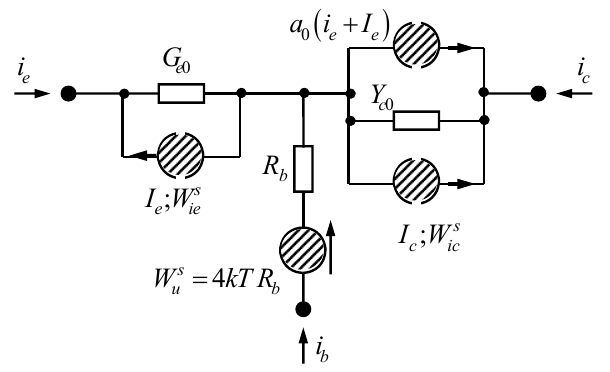
\includegraphics[width=.3\textwidth]{content/hfcomp/pictures/bjt_noise_circuit.png}
\begin{align*}
    &i_e = I_{ee} \left[\exp\left(\dfrac{q_e u_{eb}}{k_B T}\right) - 1\right] \quad \text{(signal current)},\\
    &W_{ie}^s =
    \begin{cases}
        4k_B T G_{e0} - 2q_e I_{ee} \approx 2k_B T G_{e0}, \quad I_{ee} \ll I_{eDC},\\
        2q_e (I_{eDC} + 2 I_{ee}) \equiv |\tilde{I}_e|^2, \quad \text{else}
    \end{cases}\\
    &W_{ic}^s = 2q_e a_0 (I_{eDC} + I_{ee}) + 2q_e I_{cc} \equiv |\tilde{I}^c|^2
\end{align*}
\subsubsection{Noise Matching}
\begin{itemize}
    \item \textbf{Goal:} Choose an internal generator impedance $Z_i=R_i + jX_i$ that minimizes the noise figure of a noisy two-port.
    \item Assume input noise sources:
        \begin{align*}
            &|\tilde{U}_{Nu}|^2 = 4k_B T_0 R_n \Delta f,\\
            &|\tilde{I}_{N}|^2 = 4k_B T_0 G_n \Delta f,\\
            &\tilde{U}_{Nc} = Z_c \tilde{I}_N, \quad Z_c=R_c + jX_c,\\
            &(\tilde{U}_{Nu}\text{ and }\tilde{I}_N\text{ uncorrelated})
        \end{align*}
    \item We get the optimal $Z_{i,\mathrm{opt}}$ minimal noise figure $F_{z,\mathrm{min}}$:
        \begin{align*}
            &R_{i, \mathrm{opt}} = \sqrt{\dfrac{R_n}{G_n} + R_c^2},\quad X_{i, \mathrm{opt}} = -X_c,\\
            &F_{z,\mathrm{min}} = 2\left[G_n R_n + \sqrt{G_n R_c + (G_n R_c)^2}\right]
        \end{align*}
    \item Circles of constant noise figure:
        \begin{align*}
            &\rho = \dfrac{Z_i - Z_{\mathrm{opt}}}{Z_i + Z_{\mathrm{opt}}^*}, \quad
            \Delta F = G_n R_{\mathrm{opt}},\\
            &F_z = F_{z,\mathrm{min}} \Delta F \dfrac{4|\rho|^2}{1 - |\rho|^2},\\
            &|\rho| = \sqrt{(F_z - F_{z,\mathrm{min}}) / (F_z + 4\Delta F - F_{z,\mathrm{min}})}\\
        \end{align*}
\end{itemize}

        \section{RF Two-Port Amplifiers}
\subsection{Biasing}
\begin{circuitikz}[
        scale=.9,
        transform shape
    ]
    \def\normalcoord(#1){coordinate(#1)}
    \def\showcoord(#1){coordinate(#1) node[circle, red, draw, inner sep=1pt,
    pin={[red, overlay, inner sep=0.5pt, font=\tiny, pin distance=0.1cm,
    pin edge={red, overlay}]45:#1}](){}}
    \let\coord=\normalcoord
    %% Comment next line to hide coordinate markers!
    %\let\coord=\showcoord 

    \draw (0,0) node[npn](Q){Q1};
    \path 
    (Q.B) \coord(B) (Q.C) \coord(C)
    (Q.E) \coord(E);
    \draw (Q.C) to[short, i<_=$I_{C,DC}$] ++(0,1) \coord(Y) to[R=$R_C$, i<_=$I_{C,DC} + I_{q}$] ++(0,2) to[short] ++(2.5,0) to[vsource, v=$U_{Bat}$] ++(0,-6.27) to[short] ++(-2.5,0) \coord(Z) to[R=$(R_E)$] (Q.E);
    \draw (Q.B) to [R=$R_B$, i<_=$I_{B,DC}$] ++(-3,0) \coord(X);
    \draw (Y) to[R=$R_2$, i_=$I_q$] ++(-3.84,0) to[short] (X);
    \draw (X) to[R=$R_1$, v=$U_{1,DC}$, i=$I_q - I_{B,DC}$] ++(0,-2.5) to[short] (Z);
    %% U_BE,DC
    \draw (Q.B) to[open, v=$U_{BE,DC}$] (Q.E);
    %% U_CE,DC
    \path (C) ++(.6,0) \coord(W);
    \path (E) ++(.6,0) \coord(V);
    %This is not proper, but whatever... it works!
    \draw[-{Stealth}] (W) to[out=290, in=70]node[right]{$U_{CE,DC}$} (V);
\end{circuitikz}
\\
Design Rules of Thumb:
\begin{align*}
    &U_{1,DC} \approx 0.15 \cdot U_{Bat} \quad (\text{but at least} >2U_{BE,DC}),\\
    &U_{BE,DC}(\mathrm{Si}) \approx \SI{0.7}{V}, \quad I_q \ge 10 \cdot I_{B,DC},\\
    &U_{E,DC} \approx \dfrac{U_{Bat}}{3..6} \quad (R_E > 0)
\end{align*}
\subsection{Stability}
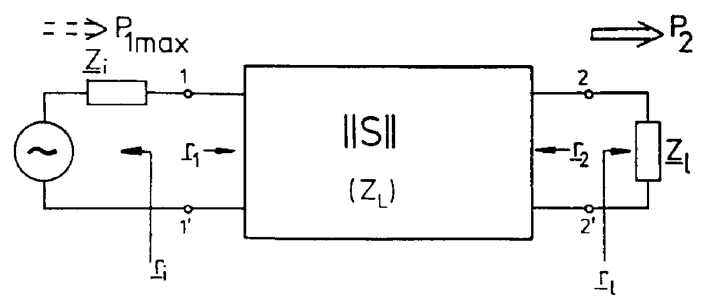
\includegraphics[width=.3\textwidth]{content/hfcomp/pictures/2-port_amplifier.png}
\begin{equation*}
    r_i = \dfrac{Z_i - Z_L}{Z_i + Z_L}, \quad r_l = \dfrac{Z_l - Z_L}{Z_l + Z_L},
\end{equation*}
\begin{equation*}
    r_1 = S_{11} + \dfrac{S_{12}S_{21}r_l}{1 - S_{22}r_l}, \quad r_2 = S_{22} + \dfrac{S_{12}S_{21}r_i}{1 - S_{11}r_i},
\end{equation*}
\begin{align*}
    g_T &= \dfrac{P_2}{P_{1,\mathrm{max}}}\\
    &=\dfrac{|S_{21}|^2 (1 - |r_i|^2) (1 - |r_l|^2)}{\left|(1 - S_{11}r_i)(1 - S_{22}r_l) - S_{12}S_{21} r_i r_l\right|^2}
\end{align*}
\begin{itemize}
    \itemsep0pt
    \item Stability Circles of Two-Port Amplifiers, with center point $\sigma$ and radius $\tau$:
        \begin{align*}
            &\text{Generator-side:}\\
            &\sigma_i = \dfrac{(S_{11} - \det(S) S_{22}^*)^*}{|S_{11}|^2 - |\det(S)|^2},\\
            &\tau_i = \left|\dfrac{S_{12} S_{21}}{|S_{11}|^2 - |\det(S)|^2}\right|\\
            &\text{Load-side:}\\
            &\sigma_l = \dfrac{(S_{22} - \det(S) S_{11}^*)^*}{|S_{22}|^2 - |\det(S)|^2},\\
            &\tau_l = \left|\dfrac{S_{12} S_{21}}{|S_{22}|^2 - |\det(S)|^2}\right|
        \end{align*}
    \item \textbf{Unconditional Stability for:}
        \begin{equation*}
            K = \dfrac{1 - |S_{11}|^2 - |S_{22}|^2 + |\det(S)|^2}{2 |S_{12}| |S_{21}|} > 1,
        \end{equation*}
        \begin{equation*}
            \text{and } |\det(S)| < 1.
        \end{equation*}.
\end{itemize}

\subsection{Unilateral Design of Two-Port-Amplifiers}
\begin{itemize}
    \item \textbf{Assume:} $S_{12} = 0$!
    \item Unilateral transducer power gain:
        \begin{equation*}
            g_{Tu,\mathrm{max},\mathrm{max}} = \frac{|S_{21}|^2}{(1 - |S_{11}|^2)(1 - |S_{22}|^2)}
        \end{equation*}
    \item \textbf{Circles of constant mismatch:}
        \begin{align*}
            &\sigma_i = \dfrac{|S_{11}| (1 - |\rho_i|^2)}{1 - |S_{11}\rho_i|^2},\\
            &\tau_i = \dfrac{|\rho_i| (1 - |S_{11}|^2)}{1 - |S_{11}\rho_i|^2}
        \end{align*}
\end{itemize}

        \section{Oscillators}
\subsection{Oscillation Condition}
\begin{itemize}
    \itemsep0pt
    \item Oscillation condition:
        \begin{align*}
            &|k| \cdot |V_u| = 1, \quad V_u = \dfrac{U_v}{U_e}, k = \dfrac{U_a}{U_v}\\
            &\varphi_v + \varphi_k = 0\text{ or }n\,2\pi
        \end{align*}
    \item Classification by feedback principle:
    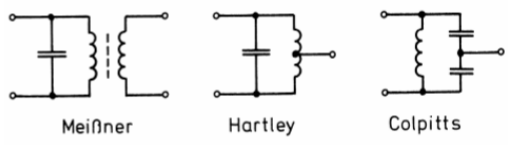
\includegraphics[width=7.5cm]{content/hfcomp/pictures/oscillator_types.png}
\end{itemize}
\subsection{Variable Oscillators}
\begin{itemize}
    \itemsep0pt
    \item Colpitts common base circuit:
        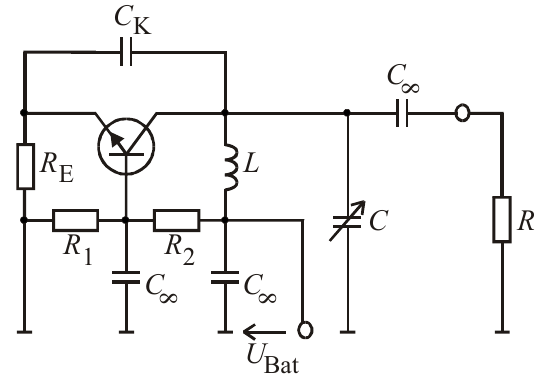
\includegraphics[width=6.5cm]{content/hfcomp/pictures/colpitts_bipolar_common_base_oscillator.png}
        \begin{align*}
            &f_S = f_T: \to \alpha \approx -\dfrac{j}{\sqrt{2}}\\
            &\omega_S C_K Z_K = \dfrac{1}{j\alpha} = \sqrt{2}
        \end{align*}
%    \item General oscillator circuit with transistor (Bipolar or FET):
%        \begin{equation*}
%            \rotatebox{-90}{%
%            $\begin{bmatrix}
%                (Y_1 + Y_3 + Y_i) & -(Y_1 + Y_i) & -Y_3 & 0\\
%                -(Y_1 + Y_i + g_m) & (Y_1 + Y_2 + Y_i + Y_0 + g_m) & -Y_2 & -Y_0\\
%                -Y_3 & -Y_2 & (Y_2 + Y_3) & 0\\
%                g_m & -(Y_0 + g_m) & 0 & Y_0
%            \end{bmatrix}
%            \begin{bmatrix}
%                U_1\\
%                U_2\\
%                U_3\\
%                U_4
%            \end{bmatrix}
%            =0
%            $}
%        \end{equation*}
\end{itemize}
\subsection{Quarz-Oscillators}
\begin{itemize}
    \itemsep0pt
    \item Oscillator stability: $\dfrac{10^{-4}}{K},\dfrac{10^{-6}}{K}...\dfrac{10^{-9}}{K}$
    \item Piezo-electric oscillator: \textit{thickness oscillator}
\end{itemize}
\begin{circuitikz}[
        scale=.9,
        transform shape]
    % ECD
    \draw (0,0) to[short, o-*] (1,0) (1,1) to[short] (1,-1);
    \draw (1,1) to[L=$L_S$, american] (3,1) to[C=$C_S$] (5,1) to[R=$R_S$] (7,1) -- (7,-1);
    \draw (1,-1) to[C=$C_p$] (7,-1);
    \draw (7,0) to[short, *-o] (8,0);
    % Labels
    \draw (.5,1.8)node[]{{\large \textbf{ECD:}}};
    \draw (.8,-1.4) to[out=270, in=180] (1,-1.6) -- (3.8, -1.6) -- (4, -1.8)node[below]{$jX$} -- (4.2, -1.6) -- (7,-1.6) to[out=0, in=270] (7.2,-1.4); 
\end{circuitikz}

\subsection{Mixer, Phase Detector}
\begin{itemize}
    \item Mixing gain (loss):
        \begin{equation*}
            g_M = 10 \lg\dfrac{P_a}{P_{1,\mathrm{max}}}
        \end{equation*}
\end{itemize}
\subsection{PLL-Circuit (Phase Locked Loop)}
\begin{itemize}
    \itemsep0pt
    \item Phase of the output signal of a controllable oscillator is locked to the phase of a reference signal by a feedback loop
    \begin{tikzpicture}[
        block/.style={
            draw,
            rectangle,
            minimum size = 1cm,
            thick,
            text centered
        },
        generator/.style={
            draw,
            circle,
            minimum size = 1cm,
            thick,
            text centered
        },
        >=Stealth,
        scale=.9,
        transform shape
    ]
    % VCO
    \node [generator](VCO) at (0,0){VCO};
    % Frequency divider 1/n
    \node[block](n) at (3,0){};
    \draw (n.south west) -- (n.north east);
    \node[above left] at (n.center){$n$};
    \node[below right] at (n.center){$1$};
    % Phase Discriminator
    \node[block](PD) at (6,0){$\varphi$};
    % Frequency Divider 1/m
    \node[block](m) at (6,2){};
    \draw (m.south west) -- (m.north east);
    \node[above left] at (m.center){$m$};
    \node[below right] at (m.center){$1$};
    % Local Oscillator
    \node[generator](LO) at (3,2){LO};
    % Lowpass Filter
    \node[block](LP) at (4.5,-2){LP};
    % Inverter
    \node[block](inv) at (1.5,-2){-1};

    % Control Loop Arrows
    \draw[->] (VCO.east) --node[below](out){} (n.west);
    \draw[->] (n.east) --node[above]{$f_0/n$} (PD.west);
    \draw[->] (PD.south) |-node[right, pos=.2]{$-U_{DC}$} (LP.east);
    \draw[->] (LP.west) -- (inv.east);
    \draw[->] (inv.west) -|node[left, pos=.75]{$U_{DC}$} (VCO.south);
    % Output Arrow
    \draw[->] (out) --node[left]{$f_0$} ++(0,1.5);
    % Reference Signal Arrows
    \draw[->] (LO.east) --node[above]{$f_Q$} (m.west);
    \draw[->] (m.south) --node[right]{$f_Q/m$} (PD.north);
\end{tikzpicture}

    \begin{equation*}
        f_0 = \dfrac{n}{m} f_Q
    \end{equation*}
    \item Digital frequency detection and division
\end{itemize}
\subsection{Two-Terminal-(1-Port)-Oscillators}
\begin{equation*}
    \text{Stability:} \dfrac{\partial Y_k}{\partial\sigma} > 0
\end{equation*}
\subsection{Oscillator Noise}
Leeson's Model for Oscillator Phase Noise:\\
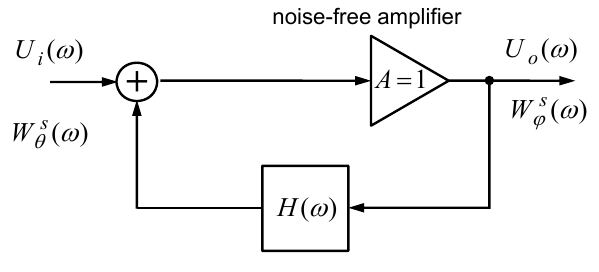
\includegraphics[width=.3\paperheight]{content/hfcomp/pictures/leeson_model_phase_noise.png}

        \section{Parametric Effects}
\subsection{Principle}
\begin{enumerate}
    \itemsep0pt
    \item At peak voltage, the capacitance is reduced (e.g. via varactor diode) $\to$ Voltage increases due to charge conservation.
    \item During zero crossing, all the energy is stored in $L$ and $C\to C_{\mathrm{max}}$ does not cause any energy change.
    \item The former steps are repeated with a rate double the frequency of the voltage oscillation to amplify the signal.
\end{enumerate}
\subsection{Nonlinear Reactance}
Most often: \textbf{capacitance diode} (Varactor)
\begin{align*}
    &C = \dfrac{\mathrm{d}q}{\mathrm{d}u_s} = C_{D0} \left(1 + \dfrac{u_s}{U_d}\right)^{-n},\\
    &U_d(\mathrm{Si}) \approx \SI{0.7}{V}, \quad n = \dfrac{1}{3}, ..., \dfrac{1}{2}\\
    &\text{Schottky diode:} \quad n = \dfrac{1}{2}
\end{align*}
\subsection{Parametric Amplifier}
\begin{equation*}
    \text{Manley-Rowe: } \sum\limits_i \dfrac{\partial \omega_i}{\partial \omega} \dfrac{P_i}{\omega_i} = 0
\end{equation*}

        \section{Transceiver Concepts and System Considerations}
\subsection{Transmitter Concepts}
\begin{enumerate}
    \itemsep0pt
    \item \textbf{Tuned Radio Transmitter:} the transmit signal is directly generated and processed. All components must support frequency tuning.
    \item \textbf{Superheterodyne Principle:} all signal process is done at a fixed intermediate frequency (IF). Other Frequencies are generated throught mixing.
\end{enumerate}
\subsection{Receiver Concepts}
\begin{enumerate}
    \itemsep0pt
    \item \textbf{Tunded Radio Receiver:} similar to tuned radio transmitter.
    \item \textbf{Superheterodyne Receiver:} HF-signal mixed down to a fixed IF for further processing. Multiple mixing stages and a \textit{lower IF} allowing for \textit{better amplification} and \textit{selectivity}.
    \item \textbf{Homodyne Receiver:} RF and LO couple phase coherently $\implies$ IF is 0. There are seperate I and Q receive channels.
\end{enumerate}
\subsection{Directive Radio}
\subsection{Satellite Radio}

	\end{multicols}
\end{document}
